\chapter{User Guide}
\label{userguide}
This chapter focuses on how to use \texnicle for common tasks. It will start with the basics and move through the most important features. A more comprehensive description of all the bells and whistles can be found in chapter \ref{reference}.

\section{Welcome Screen}
\label{userguide.welcome}
The welcome screen is shown in Figure \ref{fig:texnicle-welcome}.
\begin{figure}[htbp]
\centering
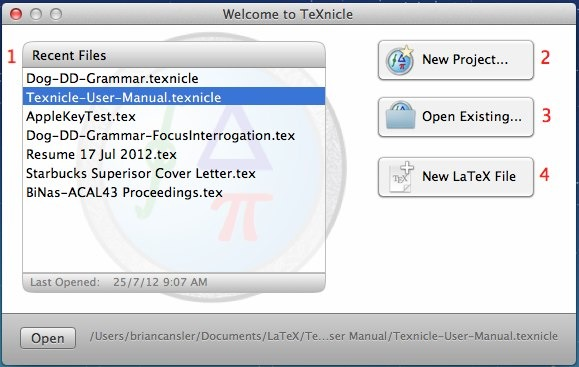
\includegraphics[width=0.75\textwidth]{TeXnicle-Images/texnicle-welcome.jpg}
\caption{\texnicle's welcome screen}
\label{fig:texnicle-welcome}
\end{figure}

When opening \texnicle for the first time, or when opening the application without loading an existing document, the welcome screen will be displayed. It has four major components:
	\begin{enumerate}
		\item \textbf{Recent Files} on the left displays a list of the files most recently opened with \texnicle. These files can be opened by selecting the file and clicking \menu{Open} at the bottom or by double-clicking the file name.
		\item \textbf{New Project\ldots} on the right will open a panel to walk the user through creating a new project. This is described in section \ref{userguide.newproject}.
		\item \textbf{Open Existing\ldots} will open the familiar Mac OS X dialogue box that will allow you to search your system for a file you wish to open.
		\item \textbf{New \LaTeX\ File} will create a new {\TeX} document. A menu will appear with template options, or you may opt to open a blank document. See section \ref{userguide.newdoc}.
	\end{enumerate}
	
\section{Quick Start}
\label{userguide.quickstart}
\begin{figure}[htbp]
\centering
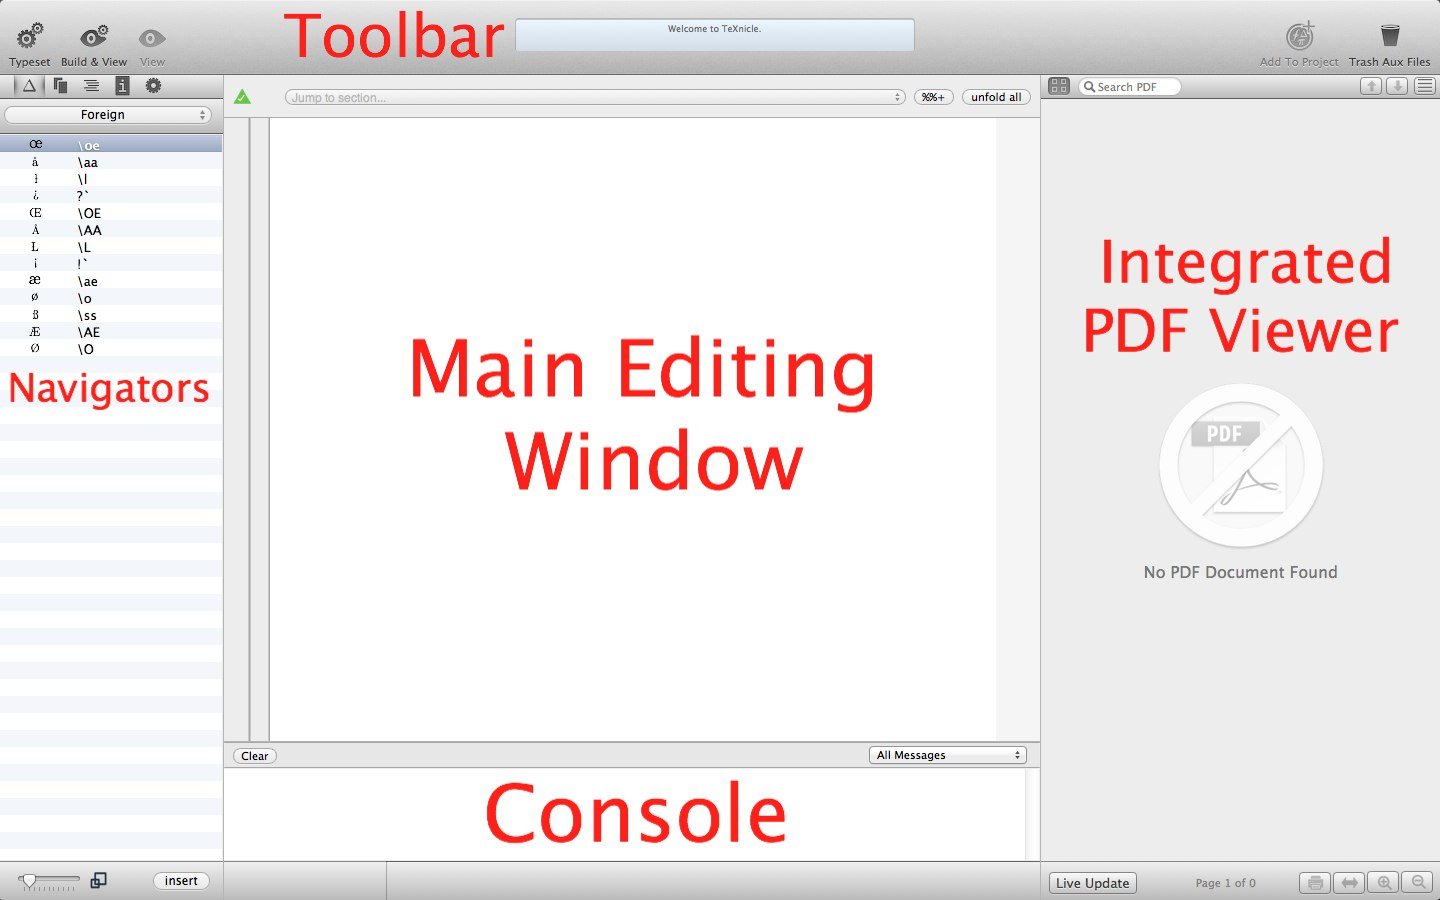
\includegraphics[width=0.5\textwidth]{TeXnicle-Images/texnicle-window.jpg}
\caption{A new window in \texnicle}
\label{fig:texnicle-newproject}
\end{figure}

The \texnicle window is divided into five major panes, which are described below. The Navigators pane, the Integrated PDF Viewer, and the Console may all be hidden and shown from the \menu{View} menu (\menu{Window} menu for the Console) at the top of the screen.

\subsection{The Toolbar}
\label{userguide.quickstart.toolbar}
Figure \ref{fig:texnicle-toolbar} shows the standard toolbar in \texnicle.
\begin{figure}[htbp]
\centering
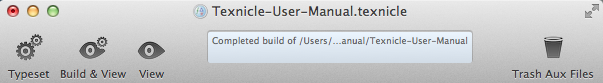
\includegraphics[width=0.75\textwidth]{TeXnicle-Images/texnicle-toolbar.png}
\caption{\texnicle's toolbar}
\label{fig:texnicle-toolbar}
\end{figure}

The toolbar includes quick access to functions that will allow you to typeset your project and open them using the built-in PDF viewer. In the center, it has a console window with status updates on the compilation of your document or project. Auxiliary files are trashed with the button on the right.\footnote{Setting defaults for files that should be trashed is done through \menu{Preferences\ldots > Typesetting > Trash}.} If the current document is not included in a project, there will also be a button in the toolbar to add that file to an existing project.

The \keys{Typeset} button (or \keys{\cmdkey + R}) will run your chosen engine on the selected document or project. This will update the Integrated PDF Viewer and (as expected) overwrite any auxiliary and output files in the project folder. The \keys{Build \& View} button will typeset your project using the chosen engine and then open the external PDF viewer. \keys{View} will simply open the external PDF viewer without typesetting.

\subsection{Main Editing Window}
%\begin{figure}[htbp]
%\centering
%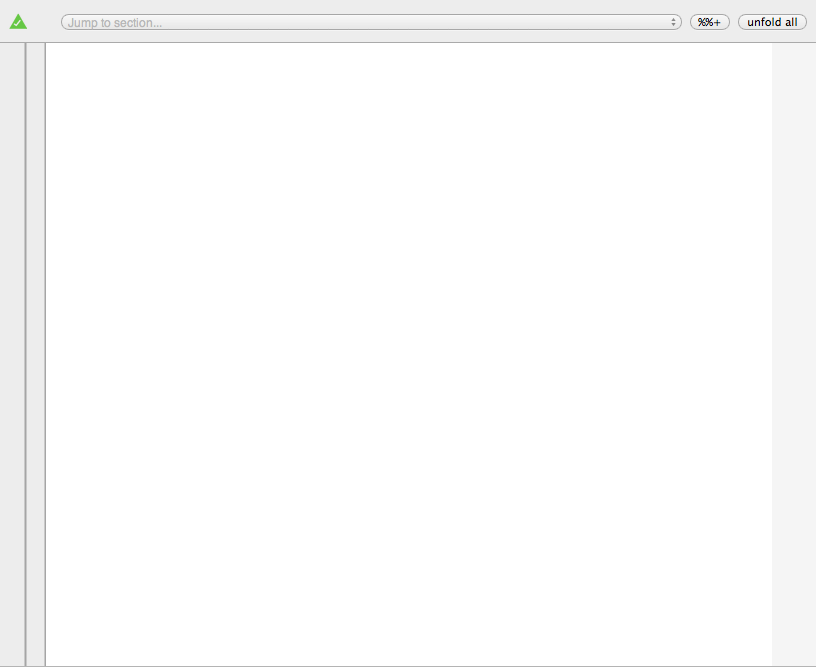
\includegraphics[width=0.4\textwidth]{TeXnicle-Images/texnicle-mainediting.png}
%\caption{The Main Editing Window in \texnicle}
%\label{fig:texnicle-mainediting}
%\end{figure}

The second part is the main editing window, located in the center. Fonts, colours, syntax highlighting, line break length, and much more can be changed under \menu{Preferences\ldots > General} and \menu{Preferences\ldots > Font \& Colors}. This is where you will write your document. In project windows, there is a bar of tabs above the main text window which shows all open documents in the project. Below the tab bar (if applicable) is a \menu{Jump to section\ldots} bar, which will allow you to jump to any section or bookmark in the open document quickly. To the left of this bar is the syntax indicator; green indicates that there are no syntax errors in the open document, while red indicates there is at least one error. Clicking the indicator will display the line numbers, descriptions, and samples of the offenses. To edit what offenses the |chktex| engine looks for, look under \menu{Preferences\ldots > Typesetting > Syntax Checking}.

\subsection{Navigators Pane}
\begin{figure}[htbp]
\begin{minipage}{0.5\textwidth}
\begin{flushleft}

\includegraphics[width=0.9\textwidth]{TeXnicle-Images/texnicle-navproj.png}
\end{flushleft}
\end{minipage}
\begin{minipage}{0.5\textwidth}
\begin{flushright}

\includegraphics[width=0.9\textwidth]{TeXnicle-Images/texnicle-navalone.png}
\end{flushright}
\end{minipage}
\caption{Icons in the Navigators pane (projects on the left, stand-alone \LaTeX\ documents on the right)}
\label{fig:texnicle-navigatorbars}
 \end{figure}
To the left of the window is the Navigators pane, which includes seven subcomponents (five in non-project windows). These are shown in Figure \ref{fig:texnicle-navigatorbars}.

\subsubsection{Project Tree}
\begin{wrapfigure}{i}{0.5\textwidth}
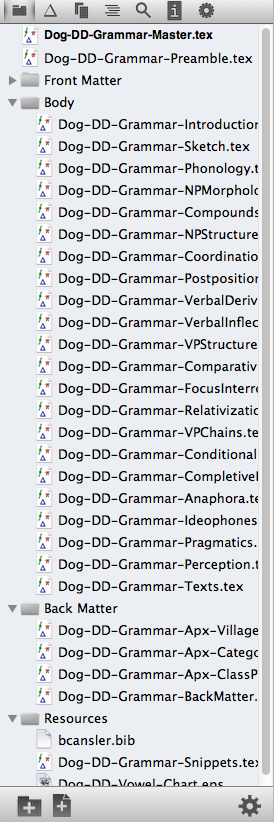
\includegraphics[width=0.48\textwidth, trim = 0 7.4in 0 0, clip = true]{TeXnicle-Images/texnicle-nav-projecttree.png}
\caption{The Project Tree in the Navigator}
\label{fig:texnicle-nav-projecttree}
\end{wrapfigure}
The first icon, a folder, is the Project Tree. It shows the tree view of your project, and so it does not appear in non-project windows. All of the project's components (files, pictures, bibliographies, folder organization, etc.)\ are listed here. The main file of the project is in bold, and it is this file that will be compiled when compiling your project. Component files are listed in unbolded black, and files with unsaved changes are greyed out. Group folders (groupings of files that appear in \texnicle but not on the disc) are grey, as in Figure \ref{fig:texnicle-nav-projecttree}; disc folders (folders that do exist on the disc) are in blue. Folders may be collapsed and expanded as needed. To move items into, out of, and between folders, simply drag and drop. \keys{\cmdkey}-click any file to set it as the main file,\footnote{Note that a project may only have one main file at a time, so setting a new main file will set it as the \emph{only} main file.} remove it from the project, rename it, or reveal it in the finder. \keys{\cmdkey}-click a folder for the same options and a few others, like adding existing files. Use the shortcut \keys{\cmdkey + \optkey + 1} to access the Project Tree quickly.

\subsubsection{Symbol Palette}
\begin{wrapfigure}{o}{0.5\textwidth}
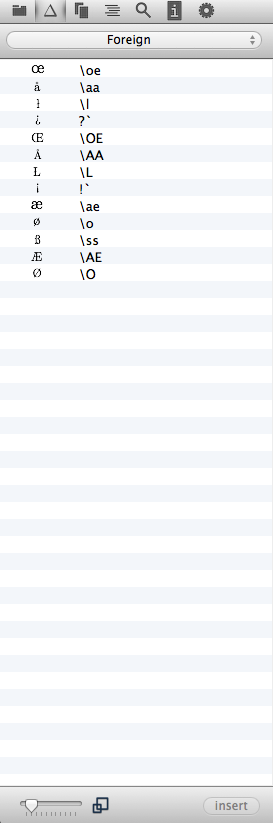
\includegraphics[width=0.48\textwidth, trim = 0 9.5in 0 0, clip = true]{TeXnicle-Images/texnicle-nav-symbolpalette.png}
\caption{\texnicle's Symbol Palette}
\label{fig:texnicle-nav-symbolpalette}
\end{wrapfigure}
The second icon is a delta symbol ($\Delta$), which opens the Symbol Palette. The category of symbols shown may be changed using the drop-down menu at the top, and the symbol may be dragged into the open document, double-clicked, or inserted using \menu{Insert} at the bottom. Categories include common foreign symbols, accents, greek letters, arrows, and a number of various mathematical subgroups. The slider at the bottom changes the size of the symbols. The Symbol Palette can be opened quickly using \keys{\cmdkey + \optkey + 2}.

\pagebreak
\subsubsection{Clippings Library}
\begin{wrapfigure}{i}{0.38\textwidth}
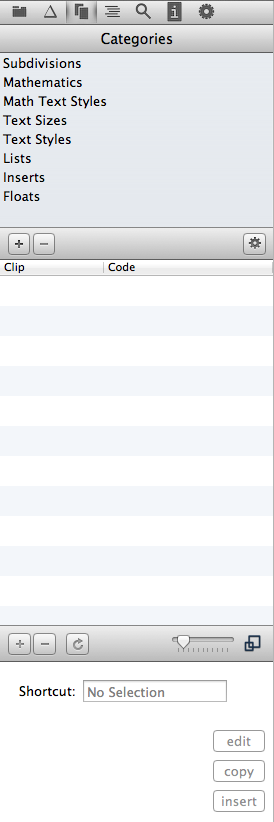
\includegraphics[height=0.8\textheight, clip=true]{TeXnicle-Images/texnicle-nav-cliplib.png}
\caption{The Clippings Library}
\label{fig:texnicle-nav-cliplib}
\end{wrapfigure}
The third component of the Navigators pane is the Clippings Library (two superimposed rectangles), which includes code fragments that you can insert into your document just like symbols from the Symbol Palette. New clippings and categories of snippets may be added from this pane, as well.

The top section of the Clippings Library lists categories of clippings. \texnicle comes pre-installed with a number of useful categories, like sectioning commands, math clips, formatting codes, and lists.

Below the categories panel is the clipping panel. Here, \texnicle will list the code clippings for a selected category (on the right) and render previews of the output (on the left). To refresh a preview, click the round arrow.

The bottom panel allows you to edit codes, copy the text of a clipping to the pasteboard, and insert clippings into your document. You may also set shortcuts here. To use a shortcut, type a |#| before the shortcut code in the main editor window; the code will turn yellow and expand by pressing \keys{\returnkey}

For more information on the Clippings Library, see \ref{reference.clippings}. To open this Navigator pane quickly, use the keyboard shortcut \keys{\cmdkey + \optkey + 3}.
\pagebreak\clearpage

\subsubsection{Document Outline}
\begin{wrapfigure}{i}{0.5\textwidth}
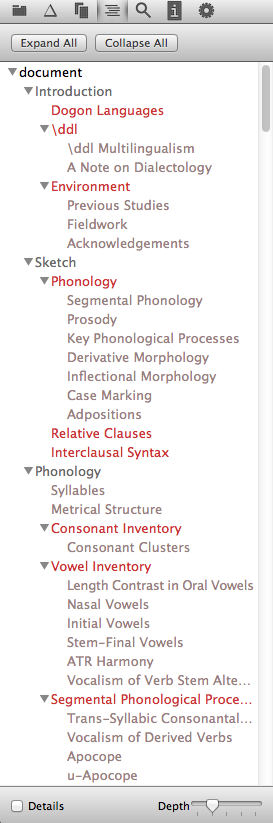
\includegraphics[width=0.48\textwidth, trim = 0 8.75in 0 0, clip = true]{TeXnicle-Images/texnicle-nav-docoutline.png}
\caption{The Navigator's Document Outline}
\label{fig:texnicle-nav-docoutline}
\end{wrapfigure}
The fourth component is the Document Outline, which shows the outline of your project or document based on sectioning commands (Part, Chapter, Section, Paragraph, and so on). This pane makes it easy to jump between sections of your entire document similarly to the \menu{Jump to section\ldots} bar at the top of the main editing window. The depth of the may be controlled using the slider at the bottom. Colours used in the outline may be edited under \menu{Preferences\ldots > Font \& Colors > Outline Colors}. To access the Navigator's Document Outline quickly, press \keys{\cmdkey + \optkey + 4}.

\subsubsection{Project Search}
\begin{wrapfigure}{o}{0.5\textwidth}
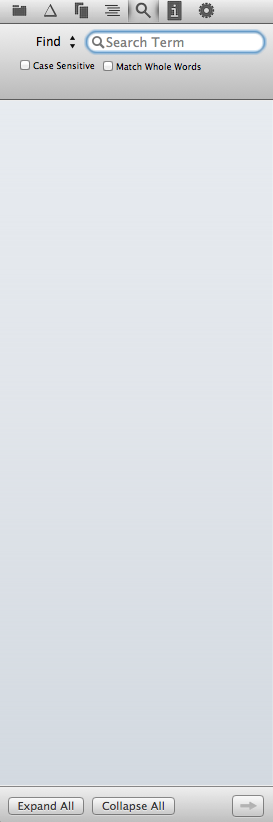
\includegraphics[width=0.48\textwidth, trim = 0 9in 0 0, clip = true]{TeXnicle-Images/texnicle-nav-projfind.png}
\caption{Project Search in the Navigator}
\label{fig:texnicle-nav-projsearch}
\end{wrapfigure}
The fifth component only appears in the Navigators pane for projects and not for stand-alone \LaTeX\ documents: Project Search. This will allow you to search all files in a project for a word or phrase. Options to conduct case-sensitive searches and to search only for whole words are available. To open Project Search quickly, press \keys{\cmdkey + \optkey + 5}.

\pagebreak\clearpage
\subsubsection{Project Information}
\begin{wrapfigure}{i}{0.5\textwidth}
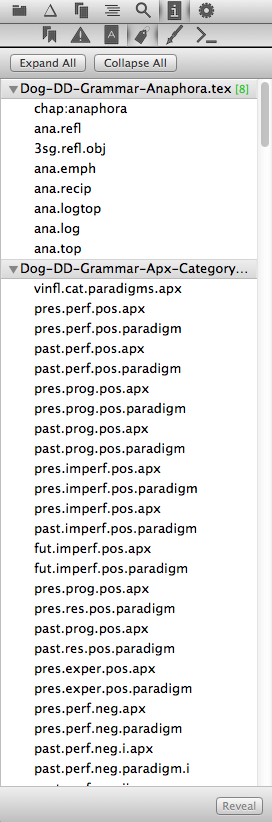
\includegraphics[width=0.48\textwidth, trim = 0 8.5in 0 0, clip = true]{TeXnicle-Images/texnicle-nav-info.png}
\caption{Project Information}
\label{fig:texnicle-nav-info}
\end{wrapfigure}
The sixth component is the Project Information tab, represented by a lowercase letter \textsl{i}. This tab appears for both projects and for stand-alone \LaTeX\ documents. This contains many important features: a list of coding errors, a list of misspelled words, a list of labels, a citation list, and a list of new commands that have been declared in each document using |\newcommand| and |\renewcommand|. In a stand-alone document, this shows everything for the open file; for a project, this shows information for every document in the project. Projects also include a tab within this section for project bookmarks

\subsubsection{Project Settings}
\begin{wrapfigure}{o}{0.5\textwidth}
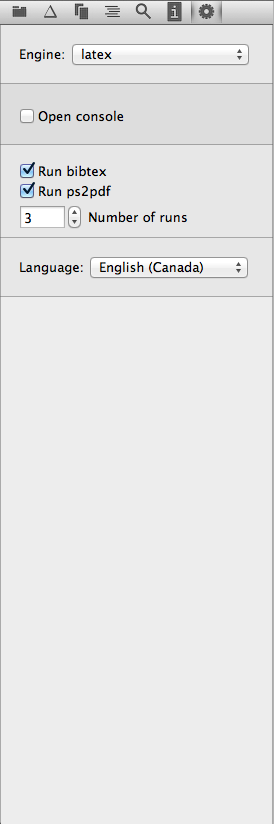
\includegraphics[width=0.48\textwidth, trim = 0 7.45in 0 0, clip = true]{TeXnicle-Images/texnicle-nav-projsettings.png}
\caption{Project Settings in the Navigator}
\label{fig:texnicle-nav-projsettings}
\end{wrapfigure}
The final component is the Project Settings tab, which appears for all documents and projects. It allows you to choose the engine used to compile your document, whether to run |bibtex| and |ps2pdf|, how many times to run |latex|, and more. The settings chosen in this panel will stay the same for a project or document regardless of any changes made in the Preferences pane. Changes in the Navigator govern the open document or project, whereas changes in Preferences govern new documents and projects.
\pagebreak\clearpage

\subsection{Integrated PDF Viewer}
\label{userguide.quickstart.pdfviewer}
\begin{wrapfigure}{i}{0.55\textwidth}
\centering
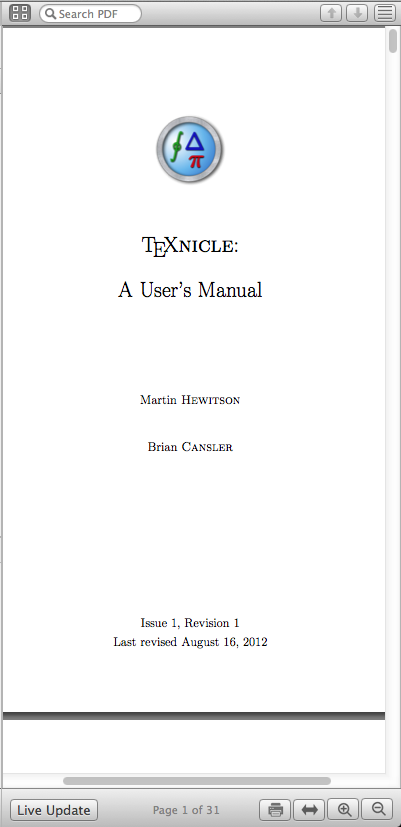
\includegraphics[width=0.53\textwidth]{TeXnicle-Images/texnicle-integratedpdf.png}
\caption{The Integrated PDF Viewer}
\label{fig:texnicle-integratedpdf}
\end{wrapfigure}
The fourth important part of the TeXnicle window is on the right: the Integrated PDF Viewer. This pane shows a live update of the document (compiled at an interval that can be set under \menu{Preferences\ldots > Typesetting}) of your document. Live updating can be turned on and off by toggling the \menu{Live Update} button at the bottom of the viewer. To update the viewer manually, click the \menu{Typeset} button on the toolbar or use the shortcut \keys{\cmdkey + R}. To typeset and view in the stand-alone PDF viewer, press \keys{\shiftkey + \cmdkey + R}. The stand-alone viewer has all of the same functions as the Integrated PDF Viewer with the sole exception of live updating: a page count of the PDF output, a search function, zoom capability, and an option to print your document.

\pagebreak\clearpage
\subsection{Console}
\label{userguide.quickstart.console}
\begin{figure}[htbp]
\centering
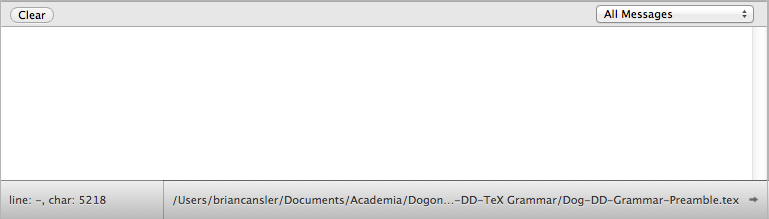
\includegraphics[width=0.65\textwidth]{TeXnicle-Images/texnicle-console.png}
\caption{The Console in \texnicle}
\label{fig:texnicle-console}
\end{figure}
The final pane is the Console pane, which appears at the bottom of the screen. When typesetting your document, this pane will show the output of the compilation commands. You can choose whether to show all messages from the console, errors only, or \texnicle messages only. Just as the Integrated PDF Viewer has a stand-alone version, you can set the Console to appear in a separate window upon typesetting under the Project Settings tab of the Navigator.

\subsection[Creating a New File]{Creating a New \LaTeX\ File}
\label{userguide.newdoc}
Whether a new {\TeX} file is created from the welcome screen, from \menu{File > New Standalone \LaTeX\ File}, or by pressing \keys{\cmdkey + N}, a new window will appear with a template selection dialogue box. Select one of the pre-existing templates from the list shown; if you choose, you may also edit the code before opening the document using the preview window below the list. Alternatively, you may create a new template by clicking the \menu{$+$} icon below the list (similarly, the \menu{$-$} icon deletes templates). The templates included are:
	\begin{itemize*}
		\item \textbf{Empty}: contains no code. It's a blank slate.
		\item \textbf{Section}: a document for a new section.
		\item \textbf{Custom}: a blank template in which you may create a custom template.
		\item \textbf{Article}: creates a document with a useful preamble for the Article class.
		\item \textbf{Book}: creates a document formatted for the Book class.
		\item \textbf{Report}: creates a new document in the Report class.
		\item \textbf{Beamer}: creates a new Beamer presentation.
	\end{itemize*}

Once you have chosen a template, enter a name for the new document and click \menu{Select}.

\subsection[Creating a New Project]{Creating a New \texnicle Project}
\label{userguide.newproject}
While \texnicle can of course work with simple \LaTeX\ documents, its true power is in its Project capabilities. A project creates a work environment with all of the files you need in one place, displaying them in an integrated tree view. Figure \ref{fig:texnicle-newproject} shows the window that appears when creating a new template. For a new empty project, you may also use the keyboard shortcut \keys{\shiftkey + \cmdkey + N}.
\begin{figure}[htbp]
\centering
\label{fig:texnicle-newproject}
\caption{Starting a new projct in \texnicle}
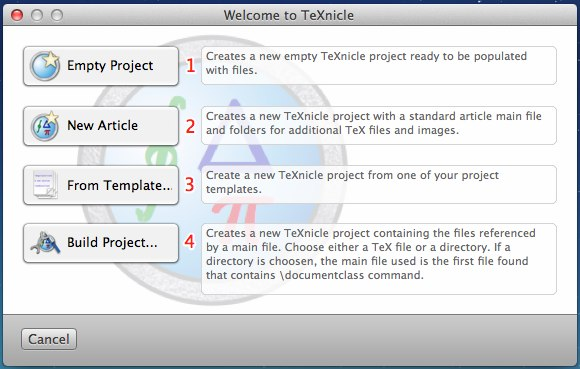
\includegraphics[width=10cm]{TeXnicle-Images/texnicle-newproject.jpg}
\end{figure}

When you opt to create a new project, you have four options:
	\begin{enumerate*}
		\item \textbf{Empty Project} creates a new empty \texnicle project to which you can add your files (or from within which you can create new files).
		\item \textbf{New Article} creates a new \texnicle project with a standard article main file and folders for additional files, images, and other resources.
		\item \textbf{From Tempate\ldots} creates a new \texnicle project from an existing project template.
		\item \textbf{Build Project\ldots} creates a new \texnicle project containing the files referenced by a main file (using |\input| and |\include| commands). You may choose either a {\TeX} file or a directory. If a directory is chosen, the main file used is the first file found with a |\documentclass| command.
		\end{enumerate*}

\texnicle will then create the project based on your selection.